\lecture{Лекция 5}{lec5}
\subtitle{Лекция 5 --- Алгебра логики. Часть 2}

\frame[plain]
{\titlepage}	% Титульный слайд


\begin{frame}
\frametitle{Алгебра логики}

\begin{center}

\Huge
Построение функции по таблице истинности
	
\end{center}


\end{frame}

\begin{frame}
\frametitle{Определения}

Для начала условимся называть конъюнкцию нескольких различных переменных или их отрицаний 
\textit{элементарым конъюнктом}. 

Например $x_1\wedge x_2\wedge \bar{x}_3\wedge x_4$. 


\end{frame}

\begin{frame}
\frametitle{Функция большинства}

Функцию большинства (\textit{голосования}) $Г(x_1,x_2,x_3)$, принимающую значение равное значению наибольшего количества аргументов, можно задать следующей таблицей:

\medskip
\begin{tabular}{|c|c|c||c|}
  \hline
  $x$  & $y$ & $z$ & $Г(x,y,z)$ \\
  \hline
   0   & 0 & 0 &  0   \\
   0   & 0 & 1 &  0   \\
   0   & 1 & 0 &  0   \\
   0   & 1 & 1 &  1 \\
   1   & 0 & 0 &  0   \\
   1   & 0 & 1 &  1 \\
   1   & 1 & 0 &  1 \\
   1   & 1 & 1 &  1 \\
  \hline
\end{tabular}

\end{frame}

\begin{frame}
\frametitle{Алгоритм построения СДНФ}

1. Выберем из таблицы все строки, в которых значение функции равно 1. 

\medskip
\begin{tabular}{|c|c|c||c|l}
  \hline
  $x$  & $y$ & $z$ & $Г(x,y,z)$ & \\
  \hline
   0   & 0 & 0 &  0 &  \\
   0   & 0 & 1 &  0 &  \\
   0   & 1 & 0 &  0 &  \\
   0   & 1 & 1 &  1 & $\leftarrow$ \\
   1   & 0 & 0 &  0 &  \\
   1   & 0 & 1 &  1 & $\leftarrow$ \\
   1   & 1 & 0 &  1 & $\leftarrow$\\
   1   & 1 & 1 &  1 & $\leftarrow$\\
  \hline
\end{tabular}

\end{frame}

\begin{frame}
\frametitle{Алгоритм построения СДНФ}

2. Каждой такой строке сопоставим элементарный конъюнкт по следующему правилу: если значение переменной $p_i$ в данной строке равно 1, то в конъюнкт входит сама переменная $p_i$, иначе её отрицание $\bar{p}_i$.

\medskip
\begin{tabular}{|c|c|c||c|l}
  \hline
  $x$  & $y$ & $z$ & $Г(x,y,z)$ & \\
  \hline
   0   & 0 & 0 &  0 &  \\
   0   & 0 & 1 &  0 &  \\
   0   & 1 & 0 &  0 &  \\
   0   & 1 & 1 &  1 & $\bar{x}\wedge y \wedge z $ \\
   1   & 0 & 0 &  0 &  \\
   1   & 0 & 1 &  1 & $x\wedge \bar{y} \wedge z$ \\
   1   & 1 & 0 &  1 & $x\wedge y \wedge \bar{z}$\\
   1   & 1 & 1 &  1 & $x\wedge y \wedge z$\\
  \hline
\end{tabular}


\end{frame}

\begin{frame}
\frametitle{Алгоритм построения СДНФ}

3. Далее все четыре конъюнкта соединяются при помощи
дизъюнкции:
$$
F(x,y,z) = (\bar x\wedge y\wedge z)\vee(x \wedge \bar y \wedge z)\vee(x \wedge y \wedge \bar z)\vee(x \wedge y \wedge z).
$$

\begin{tabular}{|c|c|c||c|l}
  \hline
  $x$  & $y$ & $z$ & $Г(x,y,z)$ & \\
  \hline
   0   & 0 & 0 &  0 &  \\
   0   & 0 & 1 &  0 &  \\
   0   & 1 & 0 &  0 &  \\
   0   & 1 & 1 &  1 & $\bar{x}\wedge y \wedge z $ \\
   1   & 0 & 0 &  0 &  \\
   1   & 0 & 1 &  1 & $x\wedge \bar{y} \wedge z$ \\
   1   & 1 & 0 &  1 & $x\wedge y \wedge \bar{z}$\\
   1   & 1 & 1 &  1 & $x\wedge y \wedge z$\\
  \hline
\end{tabular}

\end{frame}

\begin{frame}
\frametitle{Алгоритм построения СДНФ}

Полученная форумла называется \textit{совершенной дизъюнктивной нормальной формой} (сокращенно СДНФ) функции голосования.
Оказывается, что $F(x,y,z)$ реализует как раз функцию голосования.
$$
F(x,y,z) = (\bar x\wedge y\wedge z)\vee(x \wedge \bar y \wedge z)\vee(x \wedge y \wedge \bar z)\vee(x \wedge y \wedge z).
$$

\end{frame}

\begin{frame}
\frametitle{Алгоритм построения СДНФ}

4. Упрощение. Используем основные правила

Поглощение:
$$ A \vee A\wedge B =A$$ \pause

Склейка
$$ x_1\wedge x_2 \wedge x_3 \vee x_1\wedge \overline{x_2} \wedge x_3 = x_1 \wedge x_3$$

Сравниваем каждый конъюнкт к каждым. Если возможно применить формулу, то упрощаем, если нет, то оставляем конъюнкт в исходной форме.

\end{frame}

\begin{frame}
\frametitle{Алгоритм построения СДНФ}

\only<1>{$$
F(x,y,z) = (\bar x\wedge y\wedge z)\vee\underbrace{(x \wedge \bar y \wedge z)}_{нет}\vee\underbrace{(x \wedge y \wedge \bar z)}_{нет}\vee\underbrace{(x \wedge y \wedge z)}_{да}.
$$}

\only<2>{$$
F(x,y,z) = \underbrace{(\bar x\wedge y\wedge z)}_{нет}\vee(x \wedge \bar y \wedge z)\vee\underbrace{(x \wedge y \wedge \bar z)}_{нет}\vee\underbrace{(x \wedge y \wedge z)}_{да}.
$$}
\only<3>{$$
F(x,y,z) = \underbrace{(\bar x\wedge y\wedge z)}_{нет}\vee\underbrace{(x \wedge \bar y \wedge z)}_{нет}\vee(x \wedge y \wedge \bar z)\vee\underbrace{(x \wedge y \wedge z)}_{да}.
$$}

\only<1>{$$
F(x,y,z) = (y\wedge z)
$$}
\only<2>{$$
F(x,y,z) = (y\wedge z)\vee (x\wedge z)
$$}
\only<3>{$$
F(x,y,z) = (y\wedge z)\vee (x\wedge z)\vee ( x\wedge y)
$$}



\end{frame}


\begin{frame}
\frametitle{Алгебра логики}

\begin{center}

\Huge
Логические элементы	
\end{center}


\end{frame}

\begin{frame}
\frametitle{Логические элементы	}

Логический элемент в электронных схемах – это устройство, реализующее ту или
иную логическую функцию. При этом логические сигналы 0 и 1 задаются разными
уровнями напряжения.

Для изображения логических схем всегда используются условные графические
обозначения элементов, описывающие только выполняемую элементами функцию и не
зависящие от его схемы. В настоящее время в мире существует несколько общепринятых
стандартов условных обозначений. 



\end{frame}

\begin{frame}
\frametitle{Логические элементы	}

Наиболее распространенными являются
американский стандарт milspec 806В и стандарт МЭК 117-15 А, созданный
Международной Электротехнической Комиссией. 

Часто в литературе используются
также обозначения в европейской системе DIN 4070. 

В отечественной литературе
условные обозначения элементов в основном соответствуют ГОСТ 2.743-82.


\end{frame}

\begin{frame}
\frametitle{Логические элементы	}

\begin{figure}[htbp] \begin{center}
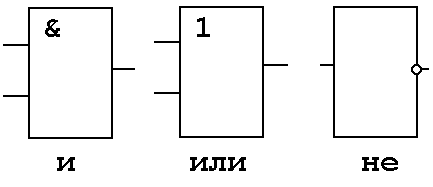
\includegraphics[height=5cm]{images/logic}

\end{center} \end{figure}


\end{frame}
\begin{frame}
\frametitle{Cхема для функции голосования	}$
F(x,y,z) = (y\wedge z)\vee (x\wedge z)\vee ( x\wedge y)$\\
\begin{figure} \begin{center}
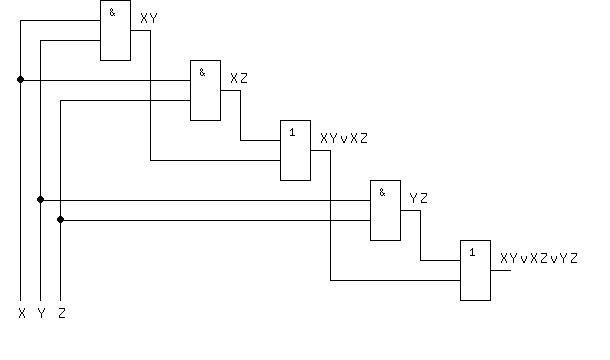
\includegraphics[height=7cm]{images/vote}

\end{center} \end{figure}


\end{frame}

\begin{frame}
\frametitle{Алгебра логики}

\begin{center}

\Huge
Как вычисления выполняются автоматически?

\end{center}

\end{frame}

\begin{frame}{Двоичные сумматоры}
\begin{itemize}
	\item \alert{Полусумматор} (HA) складывает два бита и получает бит \alert{сумма} и бит \alert{перенос} разряда.
	\item \alert{Сумматор} (FA) складывает два бита с учетом переноса разряда от предыдущего действия и получает бит \alert{сумма} и бит  \alert{перенос} разряда для следующего сложения. (разобрать самостоятельно)
\end{itemize}
\end{frame}


\begin{frame}{Полусумматор}
\begin{center}
\begin{tabular}{|c|c|c|c|}
	\hline
	\multicolumn{2}{|c|}{Вход} & \multicolumn{2}{c|}{Выход} \\
	\hline
	$x$ & $y$ & Сумма (s) & Перенос  (w) \\
	\hline\hline
	0   & 0   & 0   & 0     \\
	0   & 1   & 1   & 0     \\
	1   & 0   & 1   & 0     \\
	1   & 1   & 0   & 1     \\
	\hline
\end{tabular}
\end{center}
\pause
\begin{itemize}
	\item $s = x \oplus y=\overline{x}\wedge y \vee x\wedge \overline{y}$
	\item $w = x \wedge y$
\end{itemize}
\end{frame}

\begin{frame}{Полусумматор:схема}

\begin{itemize}
	\item $s = x \oplus y=\overline{x}\wedge y \vee x\wedge \overline{y}$
	\item $w = x \wedge y$
\end{itemize}

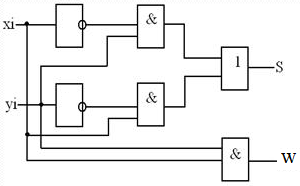
\includegraphics[height=5cm]{images/hs}
\end{frame}